\documentclass[../main.tex]{subfiles}

\begin{document}
\section{Simulation}\label{sec:simulation}
\subsection{Introduction}
Now, with all the ingredients in place, we can proceed to simulate the propagation of trajectories of some satellites.
Summarizing all the perturbations considered in this project, we have that the position $\vf{r}$ and velocity $\vf{v}=\dot{\vf{r}}$ of the satellite will be governed by the following system of differential equations:
\begin{equation}
  \begin{cases}
    \dot{\vf{r}}=\vf{v} \\
    \dot{\vf{v}}=\vf{a}_{\mathrm{GP}} + \delta_{\mathrm{D}}\vf{a}_{\mathrm{D}}+\delta_{\mathrm{R}}\vf{a}_{\mathrm{R}}+\delta_{\mathrm{sun}}\vf{a}_{\mathrm{sun}}+\delta_{\mathrm{moon}}\vf{a}_\mathrm{moon}
  \end{cases}
\end{equation}
where $\vf{a}_{\mathrm{GP}}=(\ddot{x},\ddot{y},\ddot{z})$ is the acceleration caused by the geopotential and $\ddot{x}$, $\ddot{y}$ and $\ddot{z}$ are given in \cref{eq:acceleration}; $\vf{a}_{\mathrm{D}}$ is the acceleration caused by the atmospheric drag; $\vf{a}_{\mathrm{R}}$ is the acceleration caused by the solar radiation pressure; $\vf{a}_{\mathrm{sun}}$ is the acceleration caused by the Sun; and $\vf{a}_{\mathrm{moon}}$ is the acceleration caused by the Moon. The coefficients $\delta_{i}\in\{0,1\}$ are used to enable and disable the different perturbations. The initial conditions of the initial value problem will be the position and velocity obtained from the TLE. In order to solve this system of 6 differential equations, we have opted to use the Runge-Kutta-Fehlberg method of order 7(8)\footnote{All the code used in this project can be found at \url{https://github.com/victorballester7/final-bachelor-thesis} (accessed on June 25, 2023).}. For the computation of the geopotential acceleration we will use the recursions of \cref{eq:partialaccelerationX,eq:partialaccelerationY,eq:partialaccelerationZ} until $n=8$.

There is, however, a significant comment to be made. In reality, the TLE sets are generated using a \emph{Simplified General Perturbations} (\emph{SGP}) model, and the data stored in the TLE does not contain the instantaneous orbital elements of the satellite, but doubly-averaged mean elements calculated to fit a set of observations \cite{celestrak,celestrakReport,sgp4OrbitDet}.
They are created with the SGP4 model\footnote{The SGP4 model is a mathematical model used to calculate the position of a satellite relative to an Earth-centered inertial coordinated system from the TLE data sets. The SGP4 model was developed by Ken Cranford in 1970. This model was obtained by simplification of the more extensive analytical theory of Lane and Cranford which uses the solution of Brouwer for its gravitational model and a power density function for its atmospheric model. \cite{matlab}} and, thus, we will use this software in order to obtain the position and velocity of each TLE.

That being said, we can proceed to show the results. We have chosen to simulate the propagation of the trajectories of satellites from very different altitudes: LEO satellites, MEO satellites and GEO satellites. \cref{fig:satellite_orbits} shows a schematic 2D representation of the different zones of study.
\begin{figure}[ht]
  \centering
  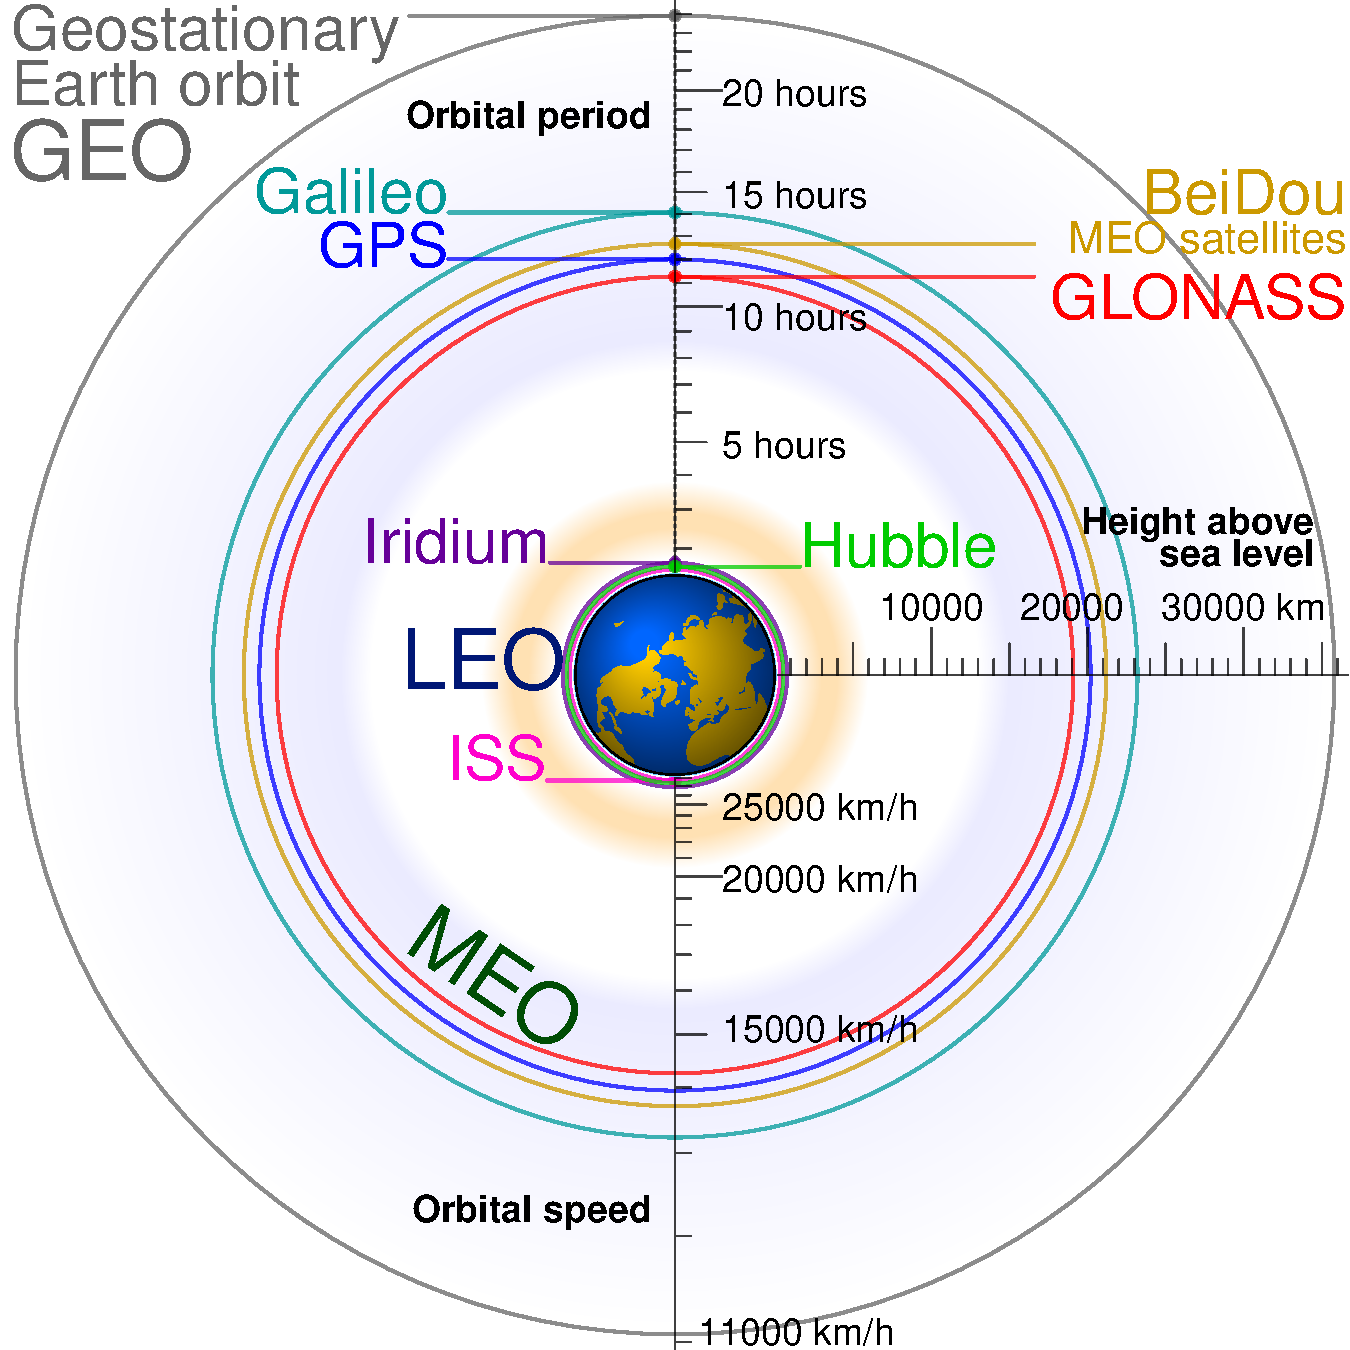
\includegraphics[width=0.55\textwidth]{Images/satellite_orbits_custom.pdf}
  \caption{Schematic 2D orbit size comparison of some orbits of satellites used in the simulation. Based on \cite{wiki:sat_orbits}.}
  \label{fig:satellite_orbits}
\end{figure}

Along this section we will compare our model with SGP4, instead of with the TLE positions directly. This approach has been considered due to the following reason. We can obtain more easily the positions of the SGP4 propagator model at any instant of time and then compare them with our propagator. Using TLE sets, we can only predict the position at certain fixed times, and that makes the comparison more difficult, specially when the TLEs are very distant in time.

\subsection{LEO satellites}
We start by simulating the propagation of the trajectories of LEO satellites. We have chosen the \emph{International Space Station} (\emph{ISS}) satellite. Its period is about 90 minutes, so it turns around the Earth about 16 times a day. That affects the propagation of errors, and as LEO satellites interact with the atmosphere and atmospheric drag is difficult to predict, they are the most problematic when it comes to propagating their trajectories. Integrating the system with a duration of 7 days, starting from January 1, 2023, we obtain the following results.
\begin{figure}[htbp]
  \centering
  \begin{minipage}[ht]{0.45\textwidth}
    \centering
    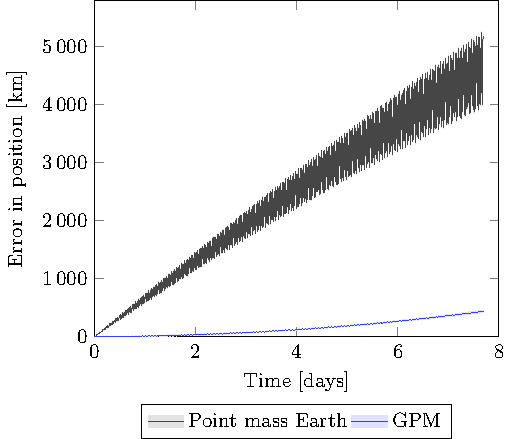
\includegraphics[width=\textwidth]{Images/simulation/ISS_pointMass_comparison.pdf}
    \caption{ISS position error when considering the Earth as a point mass or as a non-homogeneous spherical distribution of mass (with the geopotential model).}
    \label{fig:ISS_point}
  \end{minipage}
  \hspace{0.0333333\textwidth}
  \begin{minipage}[ht]{0.45\textwidth}
    \centering
    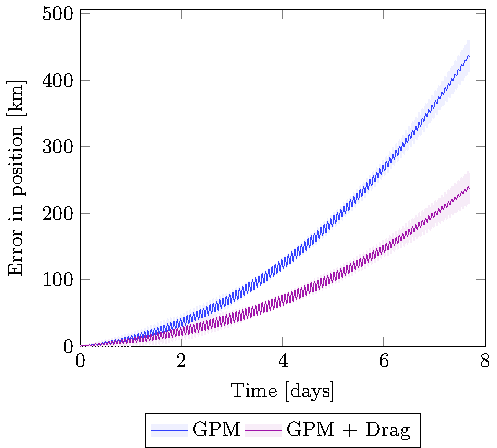
\includegraphics[width=\textwidth]{Images/simulation/ISS.pdf}
    \caption{Propagation of the ISS satellite when considering only the geopotential model for the Earth and the atmospheric drag.}
    \label{fig:ISS}
  \end{minipage}
\end{figure}

Let's make the plots clearer. The left-hand side plot has been made in order to emphasise the improvement in the approximation of the orbit obtained when considering the geopotential model (GPM) with respect to just considering the Earth as a point mass. The right-hand side plot shows two curves, which represent the errors of the position of the ISS (with respect to the SGP4 model) when considering only the geopotential model of the Earth or considering also the atmospheric drag.

In these plots, and all that will follow, each error curve will be whithin a shaded region in a lighter version of the same color. This shaded region has a vertical width which is equal to twice the linearly interpolated difference between the SGP4 propagation and the real orbit given by TLEs at specific points in time. Its goal is to give the maximum variation that our error curve would have if it was the difference between our propagation and the real orbit, instead of the difference between our propagation and the SGP4 one.

We see that, even not having a precise description of the term $C_\mathrm{D}\frac{A}{m}$ in the drag expression, we still decrease notably the error of the position of the satellite when considering the atmospheric drag. During the integration we have assumed a constant value of $C_\mathrm{D}=2.2$, which in basis of \cite{montenbruck}, is reasonable for such conditions, and we have computed the area-to-mass ratio $\frac{A}{m}$ using the mean of the $B^*$ coefficients (see \cref{tab:TLE}) of all the TLEs of the ISS and the formula:
\begin{equation}
  \frac{A}{m}=\frac{2 B^*}{\rho_0 C_\mathrm{D}}
\end{equation}
In this formula, $\rho_0=0.157\ \kg/(\m^2 \cdot R_\oplus)$ is the reference air density, and $R_\oplus=6378.1363\ \mathrm{km}$ is the reference Earth radius. The units of $B^*$ in the TLE sets are $1 / R_\oplus$.

As the ISS, and other LEO satellites, are far from the Moon and Sun, their influence is negligible for our purposes, and we have not graphically represented them, as their error curves would overlap the purple curve.

\subsection{MEO satellites}
As the Harris-Priester model for the density of the atmosphere is not valid for altitudes higher than 1000 km, in MEO satellites, we have not considered it. Instead, the gravitational pull of the Moon and the Sun is considerably high there, namely perturbing the acceleration of the satellite by a factor of $10^{-6}$ (in SI units), large enough to be considered. The solar radiation pressure is also considered, but we will see that the results are not as good as expected, probably due to the inaccuracy of the model used for it.

This time we have chosen the satellite Sirius-3 and one satellite from the Galileo constellation, namely Galileo-20. The results are shown in \cref{fig:Sirius,fig:Galileo}.
\begin{figure}[ht]
  \centering
  \begin{minipage}[ht]{0.45\textwidth}
    \centering
    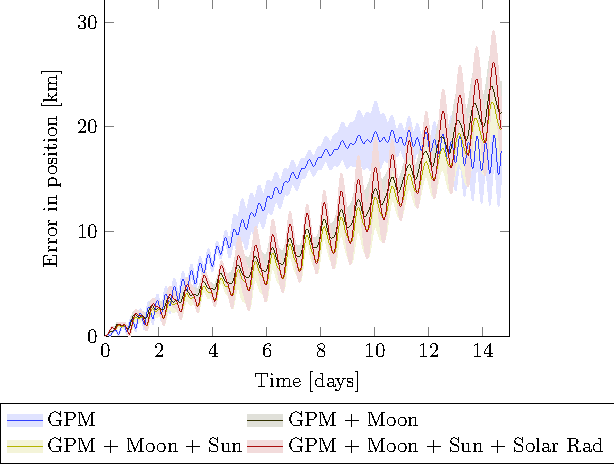
\includegraphics[width=\textwidth]{Images/simulation/SIRIUS.pdf}
    \caption{Propagation of the Sirius-3 satellite considering the perturbations from the Moon, the Sun and the solar radiation pressure.}
    \label{fig:Sirius}
  \end{minipage}
  \hspace{0.0333333\textwidth}
  \begin{minipage}[ht]{0.45\textwidth}
    \centering
    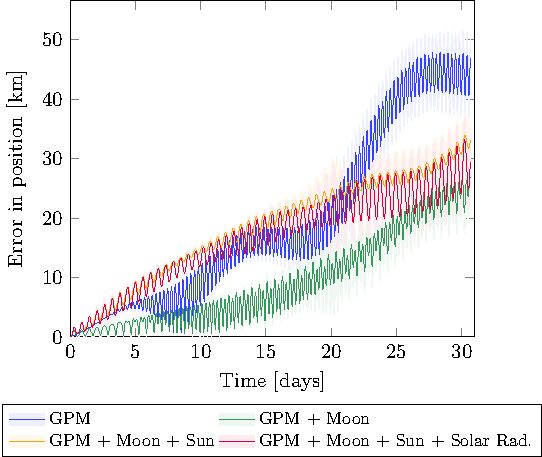
\includegraphics[width=\textwidth]{Images/simulation/GALILEO.pdf}
    \caption{Propagation of the Galileo-20 satellite considering the perturbations from the Moon, the Sun and the solar radiation pressure.}
    \label{fig:Galileo}
  \end{minipage}
\end{figure}

Let's comment the results. First note the change in duration of the integration with respect to the LEO satellites and also the decrease in magnitude of the error. These satellites travel at significantly lower speeds, completing approximately two orbits per day. As a result, the integration time can be much longer and the errors obtained are still comparable. The color codes are the same as the one in the previous plots.

We observe two very distinct results. On the one hand, errors on the Sirius-3 satellite seem to decrease when adding the Sun and Moon into the equations during the first days, although from the beginning of the 12-th day onwards, the blue curve is below the other three, but increasing its oscillations with time.
% \begin{figure}[ht]
%   \centering
%   \centering
%   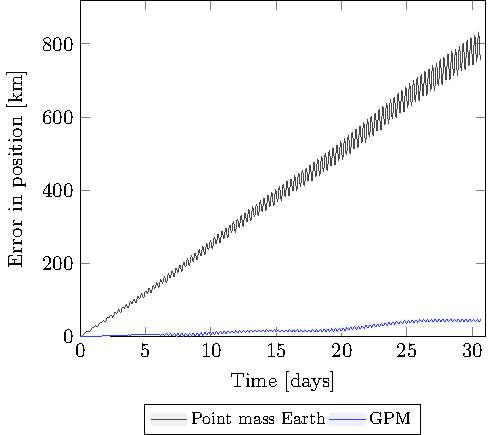
\includegraphics[width=0.45\textwidth]{Images/simulation/GALILEO_pointMass_comparison.pdf}
%   \caption{Galileo-20 position error when considering the Earth as a point mass or as a non-homogeneous spherical distribution of mass (with the geopotential model).}
%   \label{fig:Galileo_point}
% \end{figure}

On the other hand, the situation of the Galileo-20 satellite is very different. The oscillations of the GPM become larger in time and adding the Moon decreases the magnitude of the error but maintains the high oscillation rate. Nevertheless, when enabling the Sun parameter in the equation, the oscillations decrease notably, although the errors in magnitude increase slightly. This could be caused by the fact that the position of the Sun, determined by a deterministic formula given in \cite{montenbruck}, is not accurate enough.

Note that, in both cases, the solar radiation pressure increases the oscillations. Similarly to the atmospheric drag case, we have assumed a constant value of $C_\mathrm{R}=1.55$ (recommended in \cite{montenbruck}) and a constant ratio $\frac{A_\odot}{m}$ for all the satellites, due to the difficulty on obtaining this data. These imperfections of our model could be having an effect on the simulations.

As a final remark, note that if we consider the point mass approximation for the Earth for MEO spacecraft, the errors obtained are still high, as shown in \cref{fig:Galileo_point}.

\subsection{GEO satellites}
Finally, we study the GEO satellite TDRS-3. The results are shown in \cref{fig:TDRS}.
% \begin{figure}[ht]
%   \centering
%   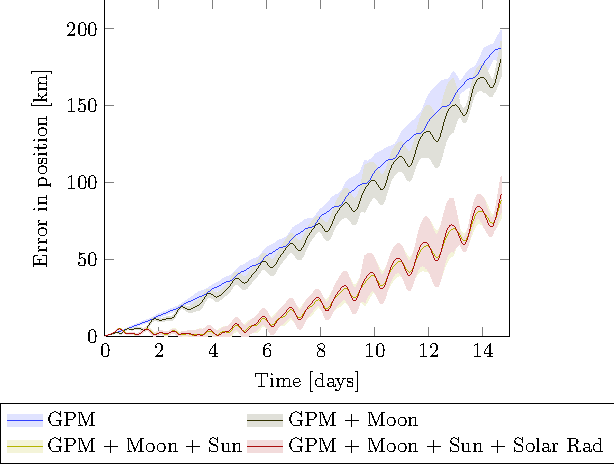
\includegraphics[width=0.5\textwidth]{Images/simulation/TDRS-3.pdf}
%   \caption{Propagation of the TDRS-3 satellite considering the perturbations from the Moon, the Sun and the solar radiation pressure.}
%   \label{fig:TDRS}
% \end{figure}

\begin{figure}[ht]
  \centering
  \begin{minipage}[ht]{0.45\textwidth}
    \centering
    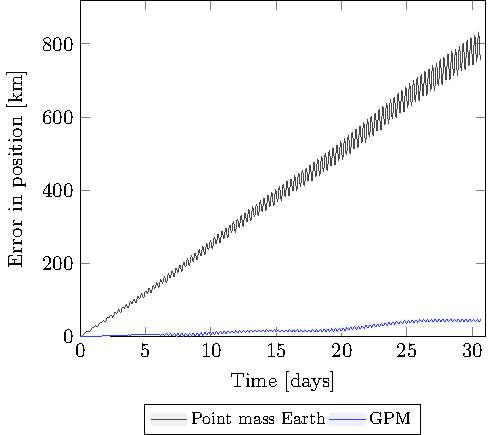
\includegraphics[width=\textwidth]{Images/simulation/GALILEO_pointMass_comparison.pdf}
    \caption{Galileo-20 position error when considering the Earth as a point mass or as a non-homogeneous spherical distribution of mass (with the geopotential model).}
    \label{fig:Galileo_point}
  \end{minipage}
  \hspace{0.0333333\textwidth}
  \begin{minipage}[ht]{0.45\textwidth}
    \centering
    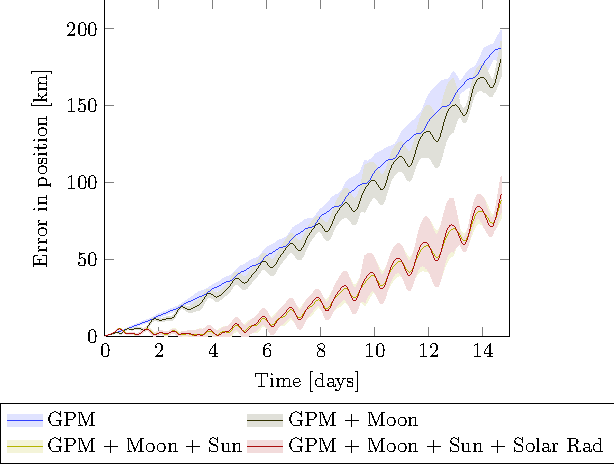
\includegraphics[width=\textwidth]{Images/simulation/TDRS-3.pdf}
    \caption{Propagation of the TDRS-3 satellite considering the perturbations from the Moon, the Sun and the solar radiation pressure.}
    \label{fig:TDRS}
  \end{minipage}
\end{figure}

This time, adding the Moon improves only about 10 km of error when comparing it to only using the geopotential model. But adding the Sun really improves the results. In particular, during the first 5 days of integration, the errors with respect to the SPG4 model remain surprisingly small.

It is known (see \cite{montenbruck}) that geosynchronous satellites require a maneuver approximately each 15 days in order to stay over a specific point above the equator with a tolerance of 0.1 degree in latitude and longitude. The fact that the width of the shaded regions decreases at around the 13th day is compatible with performing a maneuver designed in order to match with its SPG4 propagation. We have no way to check this, but it is reasonable to consider given that the SPG4 propagator is commonly employed in automatic processing to maintain a database of orbiting objects around the Earth.

\subsection{General conclusions}
On the whole, we have seen how different perturbations affect spacecraft dynamics. In particular, we have observed that the Moon and Sun gravitational attraction become noticeable in MEO an GEO satellites, whereas the atmospheric drag is only important in LEO satellites. In all the cases studied, solar radiation pressure has increased the oscillations of the errors, and therefore, for an extension of this work, it would be interesting to consider more accurate models for solar radiation pressure. The model considered for atmospheric drag is also very simple; considering a more realistic one could also improve the results of this work.

We have not considered the gravitational interaction of other planets, namely Venus, Mars and Jupiter, with the satellites in our simulations. This is because, for our purposes, the influence of other planets on the satellites is negligible due to their large distances from Earth (see \cite{montenbruck}). In particular, for the date January 1, 2023, which is approximately the initial time of all our integrations, Jupiter was located at a distance of 1.5 AU from Earth. This distance is greater than the distance between the Earth and the Sun, and Jupiter's mass is also much smaller compared to the Sun. Because of that, the gravitational effect of Jupiter is not significant in our simulations, and the same applies to the other planets. In fact, the contribution of all these three planets was of the order of $10^{-11}\ \mathrm{m/s^2}$ for MEO satellites, which is negligible when comparing it with the order of magnitude of the perturbations of the Moon and the Sun ($\sim 10^{-6}\ \mathrm{m/s^2}$).
\end{document}
